\label{ch:desing}
\chapter{Diseño e Implementación}

\section{Limitaciones técnicas}
\label{sec:limitaciones}
Como parte del diseño de la solución, se inicia con una etapa exploratoria. En
esta se anotan manualmente varias aplicaciones de Android, y se identifican
limitaciones del lenguaje Jif para anotar código de la API de Android.
Tales limitaciones son adicionales a las características del lenguaje Java no
reconocidas por Jif, a continuación se describen tanto las encontradas, como las
especificadas en el manual de referencia de Jif.

-\textit{Características del lenguaje Java no soportadas por jif}\newline
Si bien, el sistema de anotaciones de Jif hace extensiones al lenguaje java,
permitiendo la evaluación de políticas de confidencialidad e integridad para
aplicativos implementados en dicho lenguaje, el manual de referencia de Jif
precisa las características del lenguaje Java no soportadas\cite{jifRef}. Estas
son:
\begin{itemize}
  \item nested classes: clases que son definidas dentro de otras clases.
  \item initializer blocks: bloques de código declarados dentro de la clase pero
  sin pertenecer a ningún método, dependiendo de si se trata de static
  initialization blocks, su código es el primero en ejecutarse, una vez se
  carga la clase; o si se trata de instance initialization blocks, su código se
  ejecutan cada vez que se crea una instancia de la clase.
\item threads.
\end{itemize} 
Partiendo de estas precisiones, aplicaciones Android que presenten tales
características son excluidas del grupo de aplicaciones a analizar(conjunto de
aplicaciones evaluables) mediante la herramienta propuesta.

% Adicional a las limitaciones de jif frente a características propias del
% lenguaje Java, tras experimentar la anotación manual de una serie de
% aplicaciones Android, se identifican varias limitaciones técnicas para la
% anotación de de las mismas. Entre las limitaciones identificadas están:\newline 

- \textit{Soporte para sobreescritura de métodos}\newline 
En la construcción de aplicaciones Android, según el componente que se esté
implementando(activities, content providers, receivers, services), se requiere
sobreescribir métodos de la clase que extienda el componente. Así, cuando se
define un componente tipo Activity, que debe extender de la clase Activiy.java, 
se sobreescriben métodos como Oncreate. Cada que se sobreescribe
un método se utiliza el statement @Override, con el cual se informa al
compilador de Java que el método es sobreescrito. No obstante, al implementar la
versión Jif de aplicaciones Android con dicho statement, el compilador de Jif
no lo reconoce. La dificultad que se presenta está en el reconocimiento del
statement(carácter @ y clase Override), y no en la sobreescritura de métodos,
puesto que Jif soporta tal característica. El soporte para la sobreescritura de
métodos es confirmado con una sencilla prueba, anotando la clase Activity.java
del framework Android (con un único método, el método Ocreate), e implementando
la versión Jif de una aplicación Android que extiende de tal clase, en la cual
se define una actividad y sobreescribe el método Oncreate.
Cuando se comenta la sentencia @Override, el compilador de Jif identifica la
sobreescritura del método y reporta comentarios para el flujo de información.\newline 
Al investigar el por qué Jif no reconoce tal sentencia, se encuentra que dentro
de las clases Java estándar soportadas por el compilador de Jif, no está
contenida la clase java.lang.Override.\newline
Las clases Java estándar pertenecientes a los paquetes io, lang, math, net y
sql; para las que el compilador Jif brinda soporte, vienen implementadas con
anotaciones en el directorio sig-src, directorio que forma parte de la
distribución del compilador de Jif con que se esté trabajando.\newline
Una alternativa para permitir el análisis de flujo de información entre métodos
que se sobreescriben, es comentar las líneas del programa que contengan la
sentencia @Override, puesto que, al no ser reconocida por el compilador de Jif,
es la generadora de errores de compilación.

- \textit{Casting entre tipos EditText y View}\newline
El framework de Android cuenta con diferentes clases para manejar las interfaces
gráficas que presenta al usuario, entre las cuales se encuentran EditText y
View. View es la clase principal para la creación de widgets, necesarios para la
implementación de componentes interactivos en las interfaces de usuario(UI).
EditText permite adicionar campos de texto editables en UI. El casting entre los
tipos de datos que representan ambas clases, se hace cuando la aplicación debe
procesar datos provenientes de campos en las interfaces del usuario, por ejemplo
como se observa a continuación:
\begin{lstlisting}
EditText editPassword = (EditText)findViewById(R.id.password);
String password = editPassword.getText().toString();
\end{lstlisting}
la interfaz de usuario(que es de tipo View) contiene un campo R.id.password, y
para manipular la información que almacena, debe ser de tipo EditText, siendo
necesario un casting de tipo View a tipo EditText. La dificultad que se presenta
con este tipo de casting es que para el sistema de anotaciones de jif no es
válido. Luego de probar con la anotación manual de ambas clases, tratando de
dar soporte a este tipo de casting, sin obtener resultados satisfactorios, se
opta por ``simular'' estos casos, es decir, si el tipo de dato de una variable
es de tipo EditText, se crea una variable tipo String con un valor determinado,
así se omite el casting y se puede analizar el flujo de información.

- \textit{Clase nested R}\newline
El framework de Android utiliza identificadores para hacer referencia a recursos
utilizados por la aplicación, recursos como strings, widgets y layouts, tales
identificadores son autogenerados en la clase R.java, allí cada recurso es
descrito como una clase individual. Al tratarse de una clase nested, la clase R
no puede ser anotada con jif. Esto puede solucionarse implementando una
versión Jif generalizada de la clase R, que contenga los recursos utilizados en
una aplicación, definidos como variables y no como clases.

- \textit{Sources y Sinks}\newline
En los preliminares para el diseño de la solución se propone utilizar SuSi
para clasificar los sources y sinks en las aplicaciones a analizar, sin embargo, partir del
extenso conjunto de sources y sinks, clasificados por SuSi para la API de
Android, implica una mayor complejidad en el análisis, puesto que, en un
aplicativo todo el código que le conforma puede hacer parte de sources o de
sinks. Adicional a lo complejo que se puede tornar el análisis, los sources y
sinks a considerar deben depender de la política de seguridad a evaluar. En ese
orden de ideas, resulta más viable tomar un subconjunto del listado proveído por
SuSi, partiendo de los sources y sinks que evalué la política de seguridad que
se defina.

- \textit{Enhanced for loop} \newline
Además de soportar la estructura de control for, el lenguaje Java permite el uso
de enhanced for, que es utilizado para simplificar la iteración en arrays y
colecciones, por ejemplo:
% \begin{lstlisting}
% char c[] = imei.toCharArray();
% for (int i = 0; i < c.length; i++) {
% 	obfuscated += c[i] + "_";
% }          
% \end{lstlisting}  
\begin{lstlisting}
for(char c : imei.toCharArray())
obfuscated += c + "_";
\end{lstlisting}
A diferencia de Java, Jif no soporta el enhanced for.\newline
Debido a que ambas sentencias de control son equivalentes, la solución que se
propone para poder analizar flujo de información en los aplicativos Android que
contengan dicha estructura de control, es generar el equivalente del programa
haciendo uso del for, de este modo se cambia la sintaxis sin afectar la lógica
del aplicativo a analizar.

- \textit{Otras limitaciones} \newline
Adicional a las limitaciones descritas anteriormente, para las cuales se propone
una solución, se identifica que Jif no soporta la sintaxis utilizada para
definir estructuras de datos HashMaps, LinkedList y Sets, que en Java se definen
de la siguiente manera:
\begin{lstlisting}
Map<String,String> hashMap = new HashMap<String, String>();
List<String> listData;
Set<String> phoneNumbers = new HashSet<String>();
\end{lstlisting}
Jif tampoco permite la definición de interfaces como argumentos de un método. El
siguiente fragmento de código  en una aplicación Android, muestra la definición
de una interfaz pasada como parámetro al método setOnClickListener.
\begin{lstlisting}
   Button button1= (Button) findViewById(R.id.button1);
   button1.setOnClickListener(new View.OnClickListener() {
   ...
   .....}  });
\end{lstlisting}
En estos casos, la dificultad está en encontrar una sintaxis que permita obtener
la versión equivalente del programa que las contenga. A lo que se suma, la falta
de documentación disponible para solventar los mismos. En consecuencia, se omite
del conjunto de aplicaciones evaluables, aplicaciones Android que requieran en
su implementación las estructuras de datos descritas.\newline

%- \textit{Paso de statements dentro de los argumentos de un método
%(\{\}):}\newline

\section{Diseño de la solución}

\textcolor{red}
{Pregunta: los siguientes tres parrafos explican que se cambió la propuesta
incial y por qué. Es adecuado clarificarlo aquí, o se debe actualizar la
propuesta inicial acorde al diseño real? Nota: Sandra recomienda que discutamos
si los cambios han sido en el diseño o en la implementación. De ello depende
dónde deben ir, es decir, si se cambian los preliminares para el diseño de la
solución o si se dejan aquí.}

En los preliminares para el diseño de la solución se consideró la siguiente
opción: Anotar un conjunto de clases de la API de Android mediante el sistema de
anotaciones de Jif, de modo que el compilador de Jif reconociera clases propias
de esa API, y por tanto, permitiese el análisis de flujo de información a través
de estas. Habiendo asegurado el reconocimiento a un
conjunto de clases de la API de Android, era tarea del desarrollador implementar
la versión Jif del aplicativo a evaluar.

Si bien, con dicha opción de diseño se aporta para que el desarrollador
Android evalúe flujos de información en su aplicación, mediante Jif; también se
incrementa su carga de programación, puesto que, al delegarle la anotación de la
aplicación a analizar, este debe pensar dos versiones. La versión .java, donde
utiliza los métodos proveídos por la API Android para definir las
funcionalidades de su aplicación; y la versión .jif, donde define las anotaciones pertinentes para
evaluar flujos de información; tarea para la cual, se requiere un conocimiento
previo del sistema de anotaciones de Jif y la implementación de aplicaciones
haciendo uso de las mismas.

En consecuencia, se opta por un diseño en que el análisis del aplicativo no
implique carga de programación adicional para el desarrollador, sino que por el
contrario, facilite la labor del análisis.\newline 
El diseño de solución consta de dos elementos fundamentales: anotaciones a la
API de Android, más el anotador que genere la versión Jif del aplicativo a
analizar, acorde a una política de seguridad previamente definida.\newline
Ambos elementos son complementarios, puesto que, por más que se genere la
versión Jif del aplicativo a analizar, si el compilador no reconoce clases
específicas de la API que allí se usan, .jif no puede ser compilado.

Así, (1) se parte definiendo la política de seguridad a evaluar
\ref{subsection:politica}, (2) se toman a consideración elementos influyentes
para verificar el cumplimiento de la política mediante Jif
\ref{subsec:consVerPol}, y finalmente, teniendo en cuenta (1) y (2), se
especifican anotaciones a la API de Android \ref{subsec:apiAnnotations} y se
definen los lineamientos del anotador \ref{subsec:anotador}.

\subsection{Definición de la política de seguridad}
\label{subsection:politica}
Detectar si una aplicación Android(perteneciente al conjunto evaluable) presenta
flujos de información entre, información con nivel de seguridad alto e
información con nivel de seguridad bajo.\newline
Detectando fugas de información catalogada con nivel de seguridad alto, vía:
canales creados durante el control de flujo del programa(flujos implícitos),
mensajes de texto y mensajes de Log.\newline 

\subsection{Consideraciones para verificar el cumplimiento de la política
mediante Jif} 
\label{subsec:consVerPol}
Teniendo definida la política de seguridad a verificar, se describen
elementos influyentes en el diseño de la solución.

\textit{Versión de la API de Android}\newline
Las aplicaciones utilizadas para los experimentos previos a la implementación
del prototipo, y las aplicaciones a anotar con el mismo, se realiza partiendo de
la versión Android 4.2.2(API Level 17).

\textit{Versión del compilador de Jif}\newline
se parte de la versión 3.4.2 del compilador de jif, para llevar a cabo tanto los
experimentos previos como el análisis de las aplicaciones anotadas por el prototipo.

\textit{Diferencia entre una aplicación Android y una aplicación Java
convencional}\newline 
En esencia, una aplicación Android es una aplicación Java con interfaces
descritas en XML, que para ser ejecutada necesita del framework de Android,
porque este le provee acceso al hardware del dispositivo y funcionalidades del
sistema.\newline 
Por otro lado, Jif permite hacer seguimiento al flujo de información de una
aplicación Java, extendiendo el lenguaje mediante labels de seguridad.\newline
Para analizar flujo de información de una aplicación Android mediante
Jif, es importante mencionar que mientras una aplicación Java convencional
cuenta con un único punto de entrada para iniciar su ejecución, esto es, la
clase principal donde se implementa el método main; una aplicación Android puede
tener más de un punto de entrada, generados a partir de los diferentes tipos de
componentes que le integren(Activity, Service, Content Provider y Broadcast
Receiver). La necesidad de interacción del usuario para activar tales puntos de
entrada varía acorde al tipo de componente, así, en el caso de componentes tipo
Activity su ejecución sólo inicia hasta que el usuario interactúe con la
actividad, y para manejar dicha interacción, la API Android provee el método
OnCreate. De otro modo, componentes tipo Service y Broadcast Receiver, inician
su ejecución a través de los métodos OnStartCommand y OnReceive,
respectivamente, sin necesidad de interacción del usuario.\newline 
{ \color{black} {Teniendo en cuenta lo anterior, se asume que la aplicación a
evaluar tiene un único punto de entrada, que depende del tipo de componente que
implemente.} }

\textit{Chequeo de excepciones tipo Runtime}\newline
En lenguaje Java las excepciones tipo Runtime tales como NullPointerException, no
son verificadas a tiempo de compilación, sin embargo, buscando evitar la
generación de canales encubiertos mediante las mismas, Jif si las verifica. 
En consecuencia, si un programa requiere excepciones NullPointerException,
ClassCastException y/o ArrayIndexOutOfBoundsException, el programador debe
declararlas en el programa, de lo contrario, el compilador de Jif genera error.
Para las aplicaciones a analizar, se espera que el desarrollador haya
especificado las excepciones necesarias.

\textit{Información considerada con nivel de seguridad alto}\newline
Para verificar el cumplimiento de la política de seguridad a evaluar se parte de
un conjunto de sources, caracterizados por dar a conocer información del usuario, 
considerada como privada o sensible. Los métodos que integran el conjunto de sources son: 
getDeviceId, getSimSerialNumber, findViewById, getLatitude, getLongitude y
getSubscriberId. Adicional a estos métodos, se incluye el tipo de dato EditText,
si y sólo si, el campo UI al que referencia corresponde a un campo tipo
textPassword, es decir, un campo que almacena contraseñas.

\textit{Canales que muestran información con nivel de seguridad bajo}\newline
La información enviada a través de mensajes de texto y la información conocida
tanto a través de mensajes de Log, como a través de canales generados por el
control de flujo del programa, tiene en común que debe poder ser conocida por
terceros. En consecuencia, se considera que estos canales deben dar a conocer
información con nivel de seguridad bajo.\newline
En el caso de mensajes de texto y mensajes de Log, se hace referencia
específicamente a las clases Log y SmsManager de la API de Android.

\textit{Evaluación del flujo de información}\newline
Para evaluar el flujo de información, se asume que todos los métodos definidos
en la clase serán invocados, y por tanto, todos son incluidos en el análisis.\newline 
Esta decisión de análisis busca evitar el paso inadvertido de flujos de
información, generados por omisión.

\textit{Acceso a métodos de sobreescritura.}\newline
Los métodos de las clases Activity, Service y BroadcastReceiver, son métodos
que se pueden sobreescribir, todo programa Android que extienda de tales clases
debe poder utilizarlos.

\subsection{Cómo funciona el sistema de anotaciones en Jif(Para
Justificar, las anotaciones propuestas)(Ubicación temporal)}
Jif es un lenguaje tipado de seguridad que extiende al lenguaje Java con labels
de seguridad, a través de los cuales se especifican restricciones de cómo
debería ser utilizada la información.\newline 
Jif está compuesto por un compilador y un sistema de anotaciones.\newline
% El sistema de anotaciones está basado en un modelo de etiquetas
% DLM(Decentralized Label Model), donde existen principals, políticas y
% labels.\newline
Para hacer seguimiento al control de flujo de información de un programa
implementado en Java, se debe implementar la respectiva versión Jif, es decir,
la versión del programa donde mediante el sistema de anotaciones se especifican
las políticas de seguridad a evaluar.\newline 
Luego, la versión Jif del programa se compila con el compilador de Jif.
Este aplica chequeo de labels(label checking)\cite{jifRef} para verificar que
los flujos de información que se generan al interior del programa, cumplen con
las políticas definidas.\newline

-DML(Decentralized Label Model)\newline
Jif basa su sistema de anotaciones en el modelo de etiquetas DLM(Decentralized
Label Model), donde se manejan tres elementos fundamentales: Principals,
Políticas y Labels.\newline
Principals: un principal es una entidad con autoridad para observar y cambiar
aspectos del sistema. Jif cuenta con una serie de principals ya
definidos, por ejemplo, Alice, Bob, Chunck, etc, que pueden ser
utilizados al momento de anotar.\newline 
Políticas: mediante políticas de seguridad el dueño de la política, que es el
principal que la define, determina qué otros principals pueden leer o
influenciar la información. Así, una política puede ser de confidencialidad o de
integridad, y se especifican de la forma: \{owner: reader list\} u
\{owner: writer list\}.\newline 
Labels: un label consiste en un conjunto de políticas de confidencialidad e
integridad. Los labels se escriben en las expresiones del progrma que se
anota(labels de seguridad), esto es métodos, variables, arrays, etc..\newline 
En sisntesís, las políticas de seguridad definen que principals pueden leer o
modificar la información, y esas políticas se expresan mediante labels.\newline

- Label Checking\newline
Para hacer seguimiento al flujo de información de un programa, el compilador de
Jif asocia un label al program counter de cada punto del programa,
progam-counter label(\underline{pc}). En cada punto del programa, el
(\underline{pc}) representa la información que podría conocerse tras la
ejecución de ese punto del programa.
El (\underline{pc}) es afectado por los labels con que se define cada sentencia
y expresión del programa, por tanto este es considerado como el límite
superior(máxima información que podría conocerse) de los labels que han afectado
el flujo de información para llegar a un determinado punto de ejecución.\newline
Adicionalmente, jif define labels que representan la información que podría
conocerse tras la terminación normal, o terminación por excepción de las
sentencias del programa. Y labels enviroments, que para cada punto del programa
determinan la forma en que se relacionan labels y principals.\newline
El valor dichos labels es verificado durante la compilación del programa, si se
detecta que no cumplen con las restricciones establecidas en la anotación del
mismo, el compilador genera error, indicando los puntos del programa que las
incumple.\newline

- Sintaxis de labels y sintaxis para anotación de sentencias en Jif\newline

En Jif, cada expresión del programa está conformada por dos partes: java type +
security labels un label.\newline

-Llamada a métodos\newline
-Implicit flows and program-counter labels\newline
- sobreescritura de métodos

\subsection{Lineamientos de anotación}
Para verificar el cumplimiento de la política de seguridad
establecida\ref{subsection:politica} mediante el sistema de anotaciones de Jif,
se requiere: (a) definir los elementos básicos de anotación, (b) definir
las anotaciones necesarias para la API de Android y (c) definir los
criterios de anotación para los aplicativos a analizar, tales
criterios se sintetizan en un anotador.

\textbf{(a)Elementos básicos de anotación}\newline
En \ref{subsec:consVerPol} se definió qué \textit{Canales muestran
información con nivel de seguridad bajo} y cuál es la \textit{Información
considerada con nivel de seguridad alto}. Ahora, para anotar la información
catalogada con uno u otro nivel de seguridad, de modo que, partiendo de tales
anotaciones se evalué la existencia de flujos de información entre información
con nivel de seguridad alto e información con nivel de seguridad bajo, lo primero
que se debe definir es quíen representa la autoridad principal del sistema(Top
Principal) y cuáles son los labels de seguridad.\newline 
Top principal (Alice): aprovechando que Jif ya trae una serie de principals
establecidos, se define que la autoridad máxima es el principal Alice. Este
principal tendrá todo el poder para actuar sobre los aspectos del
sistema.\newline 
Label de seguridad con nivel de seguridad alto (\{Alice:\}): en base al top
principal, se define el label de seguridad que expresa el mayor nivel de
seguridad. Las variables con nivel de seguridad alto deben ser anotadas
con tal label de seguridad, ya que esté epecífica que la información
contenida en la variable solámente podrá ser Accedida por el Top
principal.\newline 
Label de seguridad con nivel de seguridad bajo (\{\}): se define un label de
seguridad que expresa el menor nivel de seguridad, para anotar información que
es de nivel de seguridad bajo y que por tanto puede ser de conocimiento público.


\textbf{(b)Anotaciones a la API de Android}\newline

\begin{figure}[h!]
	\begin{center}
	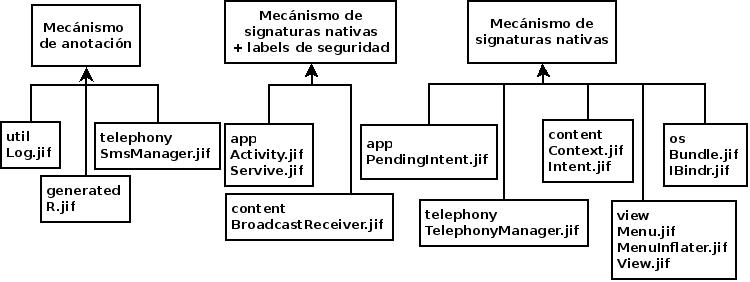
\includegraphics[width=12cm]{annotationsMechanims.jpeg}
	\end{center}
	\caption{Mecánismos de anotación para clases de la API.}
	\label{fig:annotationsMechanims}
\end{figure}

- Anotaciones para \textit{Canales que muestran información con nivel de
seguridad bajo}: para controlar el flujo de información que se envía hacia
\textit{Canales que muestran información con nivel de seguridad bajo}, es
necesario anotar la definición de los métodos de las clases Log y SmsManager de
la API Android, de manera tal, que se controle el nivel de seguridad de los
argumentos con que se invocan. Por consiguiente, en la definición del método el
AL del parametro que recibe la información a mostrar(logs) o la información a
enviar(sms), se anota con el label de seguridad bajo(label público\{\}). Con
esto se garantiza que la información se muestra o envía, si y sólo si el nivel
de seguridad del argumento con que se invoca el método es público. Por ejemplo,
si el método se llama con información anotada con label de seguridad alto, se
genera error en la compilación del programa que le llama.\newline 
El resto de labels del método BL y AL se anotan con el top principal. Al anotar
el BL con el top principal, se permite que el método sea invocado desde
cualquier punto de un programa. 
Para el resto de labels de los argumentos XXX\newline
% cualquier punto de un programa que sea igual o menor de restrictivo que el
% principal Alice, esto se traduce en que podrá ser invocado desde cualquier punto
% de un programa, lo cual es correcto porque lo que se busca el evitar que se
% envíe información considerada con nivel se deguridad alto y no, evitar que el
% método sea utilizado. Poner ejemplo XXXX?\newlie
- Anotaciones para metódos de sobreescritura: en \ref{subsec:consVerPol},
también se definieron las clases de la API para las que se debe soportar el
\textit{Acceso a métodos de sobreescritura}(Activity, Service y
BroadcastReceiver). La anotación para la definicíon de tales métodos se basa en
los siguientes criterios: (1)reglas de Jif para la sobreescritura de métodos y
(2)desde dónde pueden ser invocados. (1) Jif exige que el nivel de seguridad del
BL del método desde donde se invoca el método a sobreescribir, no debe ser menos
restrictivo que el BL de la definición de tal método(Cómo se traduce qué es más
restrictivo y que es más restrictivo? Definiciones previas).
(2) la sobreescritura de métodos se debe poder utilizar desde cualquier aplicativo que
extienda de las clases Activity, Service y BroadcastReceiver.\newline
Para cumplir con (1) y (2), los métodos que requieren ser sobreescritos se
definen con BL público(\{\}). De este modo los aplicativos desde dónde se
invocan los métodos a sobreescribir deben tener igual BL.

- Adicional a las clases de la API (Log, SmsManager, Activity, Service y
BroadcastReceiver), es necesario brindar soporte a un conjunto de clases que
representan librerias importadas por los aplicativos a analizar.(Estas
son)Brindar soporte significa que deben ser reconocidas por el compilador Jif.

% Y para poder integrarlas al conjunto de clases reconocidas por el compilador
% de Jif, basta con recurrir a signaturas nativas. Mediante el uso de signaturas
% nativas es posible incluir clases Java ya existentes. Tal mecanismo consiste en
% implementa una versión Jif de las clase fuentes, en la qué sólo es necesario
% declarar constructores y cuerpo de los métodos a utilizar.
% 
% Ahora, para incluir clases Java ya existentes es posible recurrir a signaturas
% nativas, con las cuales se implementa la versión Jif de las clases fuentes, esto
% es, declarando constructores y cuerpo de los métodos a utilizar.
- Integración de clases de la API de Android a las clases reconocidas por el
compilador de Jif:\newline
Definidos los criterios de anotación para las clases de la API, a las cuales se
debe implementar su respectiva versión Jif. Se definen los mécanismos a utilizar
para implementar tal versión. Además del mecanismo de anotación completa en que
se basa la implementación de aplicativos en Jif(mecanismo de anotación), el
compilador provee un mecanismo que permite reutilizar código de clases Java ya
existentes, para esto, se recurre a signaturas nativas. Así, se implementa una
versión Jif de una clase Java ya existente, en la que se declaran signaturas
nativas proveídas por Jif, constructor y métodos necesarios de la
clase(mecanismo de signaturas nativas).
Dependiendo de las implicaciones que pueda tener para el análisis de flujo de información del
sistema, a la versión simplificada puede específicar u omitir labels de
seguridad(mecanismo de signaturas nativas más labels de seguridad).\newline 
Para el presente caso y de acuerdo a los criterios de anotación previamente
establecidos las clases a implementar mediante uno u otro mecanismo, son
ilustrados en la siguiente figura \ref{fig:annotationsMechanims}.\newline
Nota: Falta decir qué las anotaciones a la API se implementan manualmente.

\textbf{(c)Criterios de anotación de los aplicativos a analizar}\newline
- Aquí se definen los criterios de anotación del aplicativo a analizar, y
partiendo de estos se define un algoritmo de anotación.\newline
- Al final describir exactamente las entradas y salidas del anotador, que es
donde se condensa el algoritmo de anotación.\newline


Para evaluar los flujos de información de una aplicación Android, de modo que
se verifique si cumplen con la política de seguridad definida
\ref{subsection:politica}; es necesario implementar su respectiva versión Jif,
esto implica que variables y métodos de la clase sean anotados haciendo uso del
sistema de anotaciones de Jif.\newline 
Ante esto, se propone un esquema de anotación enfocado a detectar flujos de
información desde: información considerada con nivel de seguridad alto,
hacia: canales considerados con nivel de seguridad bajo.\newline 
Retomando definiciones previas:\newline
- \textit{(a)Elementos básicos de anotación}\newline
Top principal (Alice), label de seguridad con nivel de seguridad alto
(\{Alice:\}) y label de seguridad con nivel de seguridad bajo (\{\}).\newline
- \textit{Canales que muestran información con nivel de seguridad
bajo}; como la anotación para los métodos que representan tales canales se realiza desde la
definición misma de los métodos en la API, los labels de seguridad para la
información a mostrar(logs) o enviar(msn), debe ser pública si realmente se pude
mostrar xxx.\newline
- \textit{Información considerada con nivel de seguridad alto}\newline
Los métodos que integran el conjunto de sources son: getDeviceId,
getSimSerialNumber, findViewById, getLatitude, getLongitude y getSubscriberId.
Adicional a estos métodos, se incluye el tipo de dato EditText, si y sólo si, el
campo UI al que referencia corresponde a un campo tipo textPassword, es decir,
un campo que almacena contraseñas. 



% \subsection{Anotaciones a la API de Android}
% \label{subsec:apiAnnotations}
% 
% \begin{figure}[h!]
% 	\begin{center}
% 	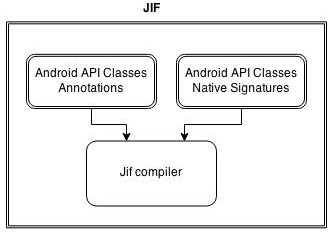
\includegraphics[width=5cm]{desingSol-steps1.jpg}
% 	\end{center}
% 	\caption{Tipos de anotación necesarias para implementar la solución.}
% 	\label{fig:desingSol-steps1}
% \end{figure}
% 
% \begin{figure}[t!]
% 	\begin{center}
% 	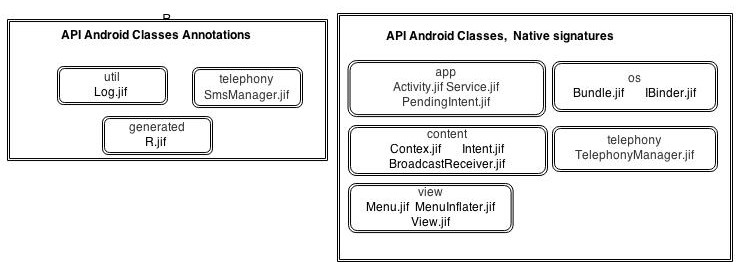
\includegraphics[width=12cm]{desingSol-step1-details.jpg}
% 	\end{center}
% 	\caption{Clases de la API a anotar.}
% 	\label{fig:desingSol-details}
% \end{figure}
% 
% El compilador de Jif tiene implementadas mediante el sistema de anotaciones Jif,
% las clases estándar del lenguaje Java para las que brinda soporte.\newline
% Ahora, para incluir clases Java ya existentes es posible recurrir a signaturas
% nativas, con las cuales se implementa la versión Jif de las clases fuentes, esto
% es, declarando constructores y cuerpo de los métodos a utilizar.
% 
% Para dar soporte a clases específicas de la API de Android se recurre a ambas
% opciones de anotación. Tal como se ilustra en la figura
% \ref{fig:desingSol-steps1}.\newline 
% El criterio para decidir que se anota de una u otra forma, depende de lo que
% represente la clase Android para verificar la política de seguridad
% establecida.\newline
% Las clases Log y SmsManager, que representan canales para conocer información,
% son anotadas de forma no nativa.\newline
% La opción de anotación nativa se utiliza
% para librerías Android, por ejemplo la clase TelephonyManager necesaria para utilizar
% el método getDeviceId.\newline
% En la figura \ref{fig:desingSol-details} se
% especifican clases de la API Android a anotar.\newline

\subsection{Diseño del anotador}
\label{subsec:anotador}
\label{subsec:pasosSol}
\begin{figure}[H]
	\begin{center}
	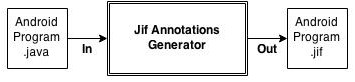
\includegraphics[width=7cm]{desingSolution.jpg}
	\end{center}
	\caption{Entradas y salidas para el generador de anotaciones.}
	\label{fig:desingSolution} 
\end{figure}

El anotador debe recibir como entrada el código fuente de la aplicación
Android(perteneciente al conjunto evaluable), para retornar su respectiva
implementación en Jif, versión que contiene las anotaciones para evaluar la
política de seguridad definida. Tal como se ilustra en la figura
\ref{fig:desingSolution}\newline 
Luego la versión obtenida se evalúa con el compilador de Jif.

A continuación, se definen los lineamientos de anotación:\newline
% \textit{Paso dos: Definir Autoridades y forma de anotación del aplicativo
% Android a analizar.}\newline
Una clase Android tendrá una Autoridad máxima(un principal), en este caso Alice,
así que, información con nivel de seguridad alto deberá pertenecer a dicha
autoridad.\newline
Jif hace seguimiento al flujo de información del programa, asociando un label
de seguridad al program counter de cada sentencia y expresión del programa,
program counter(pc) label. Este pc es afectado por el label de seguridad que se
especifique en la declaración de variables y métodos\ref{subsec:JifSintax}. 
Partiendo de que Jif se fundamenta en labels de seguridad para hacer seguimiento
al flujo de información del programa, es necesario definir los labels a
anotar para métodos y variables del programa.\newline
En el caso de variables con nivel de seguridad  alto, la anotación debe
ser:\newline
\emph{ type\{Alice:\} varName; }\newline
Para el resto de variables, entran a jugar las anotaciones definidas por Jif
acorde al contexto donde están definidas.\newline
Ahora en el caso de los métodos, la anotación varía según si el método debe
influenciar(acceder, modificar) o no, información anotada con nivel de seguridad
alto.

En base a lo anterior, se define un algoritmo de anotación que se condensa en un
generador de anotaciones; y está fundamentado en las siguientes
definiciones:\newline \textit{Definición A:} anotación de variables con nivel de
seguridad alto:\newline modifier type\{Alice:\} varName;\newline 
\textit{Definición B:} métodos que se sobreescriben. El sistema de anotaciones
de Jif exige que el nivel de seguridad del método desde donde se invoca la
sobreescritura de un método, no debe ser menos restrictivo que el método a
sobreescribir, y los métodos a sobreescribir deben poder ser invocados desde
todo programa Android, siguiendo con este principio, y buscando que jif no
limite el flujo de información, estos métodos deben ser anotados con BL
público(\{\}).\newline 
\textit{Definición C:} anotación de métodos con sources\newline
\textcolor{red}{La definición de los terminos etá en: Sintaxis de anotación en
Jif \ref{subsec:JifSintax}, debo recordar lo que significan, o remito el lector
a dicha sección?}\newline
Los labels para la definición del método\textcolor{red}{(BL, EL,
AL )}se anotan de la siguiente manera:\newline modifier type
nameMethod\textit{\{Alice:\}} type\textit{\{Alice:\}}
( arg1,.....type\textit{\{Alice:\}}argn ) \{\}\newline Si dentro del método se
definen arrays, sus respectivos BL y SL, deben ser anotados así: modifier type\{Alice:\}[ ]\{Alice:\}\newline
\textit{Definición D:} anotación de métodos que no reciben información del
source. 
nameMethod\textit{\{\}}(
type\textit{\{Alice:\}}arg1,.....type\textit{\{Alice:\}}argn ) \{\}\newline
Teniendo claras las anteriores definiciones, los pasos para el algoritmo son los
siguiente:\newline
(1) Identificar sources de la clase. Si se encuentran sources continuar con
los pasos (2) a (4), sino, continuar con paso (2) y aplicar definiciones B y
D.\newline
(2) Identificar el total de métodos de la clase.\newline
(3) Del total de métodos listar los que son invocados con el source.\newline
(4) Del total de métodos listar los que no son invocados con el source.\newline
(5) Aplicar definición C a listado del paso(3).\newline
(6) Aplicar definición D a listado del paso (4).\newline
(7) Aplicar definición B. \newline
(8) Aplicar definición A a listado del paso (1).

\subsection{Descripción implementación prototipo}
-Diagrama de clases o descripción\newline
En la sección \ref{sec:diagramaClass} de los anexos, se incluye el diagrama de
clases para la implementación del anotador.\newline

El anotador consta de cinco clases 



